\section{Dynamik}

\textbf{Dynamisches Modell}: Beschreibt Zusammenhang zwischen Antriebs- und Kontaktkräfte, welche in einem mechanischen Mehrkörpersystem auftreten und deren resultierenden Beschleunigungen und Bewegungen\\

\textbf{Allgemeine Bewegungsgleichung}:
$$\boldsymbol{\tau}=M(\mathbf{q})\mathbf{\ddot{q}}+C(\mathbf{q},\mathbf{\dot{q}})\mathbf{\dot{q}}+g(\mathbf{q})+\varepsilon(\mathbf{q},\mathbf{\dot{q}},\mathbf{\ddot{q}})$$
mit:
\begin{itemize}
	\item $\mathbf{q},\mathbf{\dot{q}},\mathbf{\ddot{q}}$: $n\times 1$ Vektor der generalisierten Koordinaten (Position, Geschwindigkeit und Beschleunigung)
	\item $\boldsymbol{\tau}$: $n\times 1$ Vektor der generalisierten Kräfte
	\item $M(\mathbf{q})$: $n\times n$ Massenträgheitsmatrix
	\item $C(\mathbf{q},\mathbf{\dot{q}})\mathbf{\dot{q}}$: $n\times 1$ Vektor mit Zentripetal- und Corioliskomponenten
	\item $g(\mathbf{q})$ : $n\times 1$ Vektor der Gravitationskomponenten
	\item $\varepsilon(\mathbf{q},\mathbf{\dot{q}},\mathbf{\ddot{q}})$: $n\times 1$ Nichtlineare Effekte, wie z.B. Reibung 
\end{itemize}
\bigskip
\textbf{Generalisierte Koordinaten}:
\begin{itemize}
	\item \textbf{Definition}: Minimaler Satz an voneinander unabhängigen Koordinaten, der den aktuellen Systemzustand vollständig beschreibt
	\item Allgemein: Roboter besteht aus $N$ Partikel. Für jeden Ortsvektor eines Partikels braucht man 3 Raumkoordinaten, insgesamt $3N$ Koordinaten, um das System zu beschreiben
	\item Partikel können sich wegen Verbindungen und Gelenken nicht unabhängig voneinander
	bewegen $\rightarrow$ Einführung von \textbf{Zwangsbedingungen}
	\item $3N$ Koordinaten lassen sich mit $k$ unabhängigen Zwangsbedingungen auf $3N-k$ unabhängige generalisierte Koordinaten $q_i$ reduzieren
	\item \textbf{Beispiel}: \textit{4/11-15}
\end{itemize}
\bigskip
\textbf{Direktes Dynamisches Problem}:  
\begin{itemize}
	\item Gegeben externe Kraft und aktueller Bewegungszustand, was ist die neue Bewegung des Systems?
	\begin{center}
		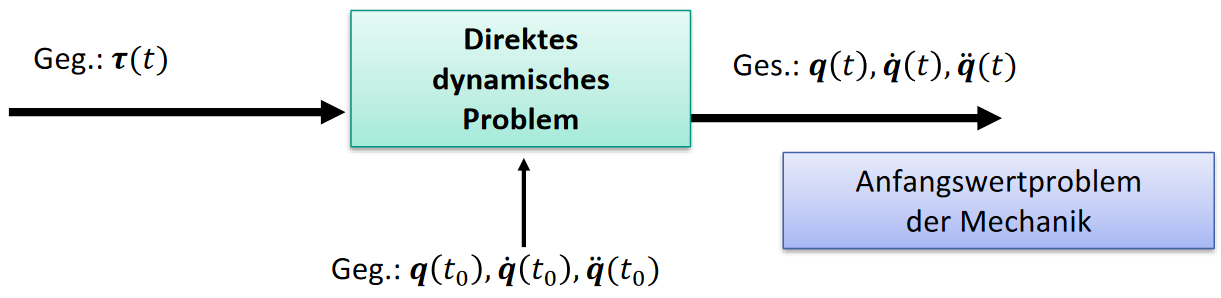
\includegraphics[width=0.7\textwidth]{images/dir-dyn.png}
	\end{center}
	\item Löse Differentialgleichung $\boldsymbol{\tau}=M(\mathbf{q})\mathbf{\ddot{q}}+C(\mathbf{q},\mathbf{\dot{q}})\mathbf{\dot{q}}+g(\mathbf{q})$ nach $\mathbf{q}(t),\mathbf{\dot{q}}(t),\mathbf{\ddot{q}}(t)$
\end{itemize}
\bigskip
\textbf{Inverses Dynamisches Problem}:
\begin{itemize}
	\item Aus den gewünschten Bewegungsparametern sollen die dazu erforderlichen Kräfte und Momente ermittelt werden
	\begin{center}
		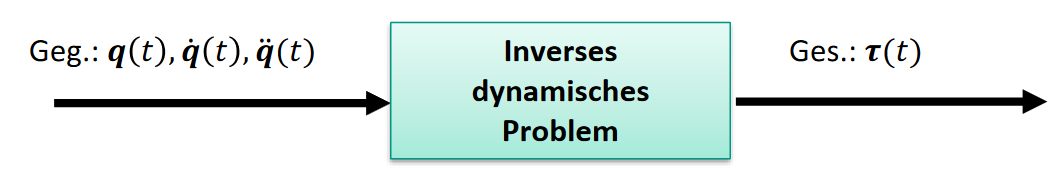
\includegraphics[width=0.7\textwidth]{images/ind-dyn.png}
	\end{center}
	\item Berechne rechten Teil der Gleichung $\boldsymbol{\tau}=M(\mathbf{q})\mathbf{\ddot{q}}+C(\mathbf{q},\mathbf{\dot{q}})\mathbf{\dot{q}}+g(\mathbf{q})$ durch Einsetzen
\end{itemize}
\bigskip
\textbf{Modellierung der Dynamik}: Versuche Terme der allgemeinen Bewegungsgleichung herzuleiten

\textbf{Methode nach Lagrange}:
\begin{enumerate}
	\item Ermittle $E_\text{kin}$ und $E_\text{pot}$
	\item Drücke $E_\text{kin}$ und $E_\text{pot}$ in generalisierten Koordinaten als \textbf{Lagrange-Funktion} aus $$L(\mathbf{q},\mathbf{\dot{q}})=E_\text{kin}(\mathbf{q},\mathbf{\dot{q}})-E_\text{pot}(\mathbf{q})$$
	\item Für jedes Gelenk $i$ ist die Bewegungsgleichung: $$\tau_i=\cfrac{d}{dt}\left(\cfrac{\partial L}{\partial \dot{q_i}}\right)-\cfrac{\partial L}{\partial q_i}$$
\end{enumerate}

\textbf{Beispiele}: \textit{4/26-35}\\

\textbf{Eigenschaften}:
\begin{itemize}
	\item Einfaches Aufstellen der Gleichungen
	\item Geschlossenes Modell, analytisch auswertbar
	\item Berechnung sehr umfangreich $\mathcal{O}(n^3)$
	\item Nur Antriebsmomente werden berechnet
\end{itemize}
\bigskip
\textbf{Methode nach Newton-Euler}:
\begin{itemize}
	\item \textbf{Newton-Euler Gleichungen}: 
	\begin{center}
		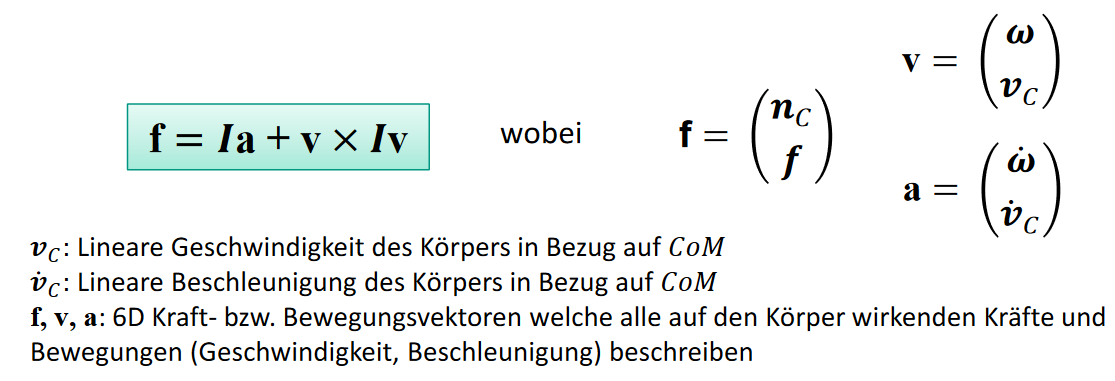
\includegraphics[width=0.8\textwidth]{images/newton-euler.png}
	\end{center}
	\item Die Beschleunigungen $\mathbf{\ddot{c_i}}$ und $\boldsymbol{\dot{\omega}_i}$ eines Armelementes $i$ hängen von den Beschleunigungen der vorhergehenden Armelemente ab
	
	$\rightarrow$ Beschleunigungen können über kinematisches Modell von der Basis zum Greifer rekursiv	berechnet werden $\rightarrow$ \textbf{Vorwärtsgleichungen}
	
	\item Die Kraft $\mathbf{f}_i$ und das Drehmoment $\mathbf{n_{C,i}}$, die auf ein Armelement $i$ wirken, hängen von den nachfolgenden Armelementen ab
	
	$\rightarrow$ Kräfte und Momente können vom Greifer zur Basis rekursiv berechnet werden
	$\rightarrow$ \textbf{Rückwärtsgleichungen}
	
	$\rightarrow$ \textbf{Rekursiver Newton-Euler Algorithmus} (RNEA)
\end{itemize}
\bigskip
\textbf{Rekursiver Newton-Euler Algorithmus}:
\begin{enumerate}
	\item Rekursive Berechnung der Geschwindigkeit und Beschleunigung jedes einzelnen Armelements $i$ von der Basis bis zum Endeffektor:
	\begin{itemize}
		\item Geschwindigkeit: $\mathbf{v_i}=\mathbf{v_{p(i)}}+\boldsymbol{\Phi_i}\mathbf{\dot{q_i}}$ mit $\mathbf{v_0}=0$
		\begin{itemize}
			\item $\mathbf{\dot{q_i}}$: Generalisierte Geschwindigkeit des Armelements $i$
			\item $\boldsymbol{\Phi_i}$: $6\times n$ Bewegungsmatrix (Abhängig vom Gelenktyp)
			\item $\mathbf{v_{p(i)}}$: Geschwindigkeit des Vorgängerelements $p(i)$
		\end{itemize}
		\item Beschleunigung: $\mathbf{a_i}=\mathbf{a_{p(i)}}+\boldsymbol{\Phi_i}\mathbf{\ddot{q_i}}+\boldsymbol{\dot{\Phi_i}}\mathbf{\dot{q_i}}$ mit $\mathbf{a_0}=-\mathbf{a_g}$
	\end{itemize}
	\item Berechnung der Kräfte/Momente jedes einzelnen Armelements $i$ mithilfe Newton-Euler:
	$$\mathbf{f_i^a}=\mathbf{I_ia_i}+\mathbf{v_i}\times\mathbf{I_iv_i}$$
	\begin{itemize}
		\item $\mathbf{f}_i^a$: Kräfte, welche aufgrund von $a_i$ auf das Armelement $i$ wirken
		\item $\mathbf{I_i}$: Trägheitsmoment des Armelements $i$
		\item $\mathbf{v_i}$: Geschwindigkeit des Armelements $i$ (in Schritt 1 berechnet)
		\item $\mathbf{a_i}$: Beschleunigung des Armelements $i$ (in Schritt 1 berechnet)
	\end{itemize}
	\item Rekursive Berechnung der Kräfte zwischen den Armelementen und der generalisierten Kräfte für den jeweiligen Gelenktyp:
	\begin{itemize}
		\item $\mathbf{f_i}=\mathbf{f_i^a}-\mathbf{f_i^e}+\sum\limits_{j\in c(i)}\mathbf{f_j}$
		\item $\boldsymbol{\tau_i}=\boldsymbol{\Phi_i^\top}\mathbf{f_i}$
		\begin{itemize}
			\item $\mathbf{f_i}$: Resultierende Kraft am Armelement $i$
			\item $\mathbf{f_i^e}$: Summe aller externen Kräfte, die an $i$ wirken
			\item $\mathbf{f_i}$: Kraft eines anliegenden Armelementes $j$
			\item $c(i)$: Menge nachfolgender Armelemente $i$ in kinematischer Kette
			\item $\boldsymbol{\Phi_i}$: $6\times n$ Bewegungsmatrix (Abhängig vom Gelenktyp)
			\item $\boldsymbol{\tau_i}$: Generalisierte Kräfte/Momente an $i$
		\end{itemize}
	\end{itemize}
\end{enumerate}

\textbf{Eigenschaften der Methode nach Newton-Euler}:
\begin{itemize}
	\item Beliebige Anzahl von Gelenken
	\item Belastungen der Armelemente werden berechnet
	\item Aufwand $\mathcal{O}(n)$
	\item Rekursion
\end{itemize}
\bigskip
\textbf{Herausforderungen der Dynamik}:
\begin{itemize}
	\item Nichtlineare Kräfte (wie z.B. Reibung) können nicht direkt modelliert werden, haben jedoch einen großen Einfluss
	\item Dynamik eines Roboters kann sich im Laufe der Zeit stark verändern z.B. durch Abnutzung
	\item Dynamik variiert stark in Abhängigkeit von der auszuführenden Aufgabe
\end{itemize}
\pagebreak